\section{Predicting blooms} \label{sec:previous}

\subsection{Introduction to previous work} \label{sec:previous_intro}
Because of the many factors influencing the dynamics of phytoplankton, attempting to describe it with a mathematical approach will result in a strongly nonlinear problem. A full dissertation would need a set of equation, each modeling the dynamics of a single species in relation to the others: this approach has been applied when dealing with the competition for resources neglecting the spatial distribution of cells \autocite{Leon1975CompetitionResources}. This has given some insights into the problem of ``plankton paradox'', that is, the unexplained variety of species of plankton occupying (apparently) the same biological niche, and has been studied from a chaotic point of view \autocite{Huisman2002OscillationsResources}. 

Another approach, aimed at modeling the spatial distribution of phytoplankton, is exemplified by \autocite{visser1997modelling}, where the reproduction of cells is neglected, the light intensity influencing the buoyancy rate. In high light conditions, the cells accumulate carbohydrates, resulting in an increased cell density; on the opposite, in low light conditions the cells utilize the carbohydrates produced, increasing buoyancy. In \autocite{medrano2013coupling}, the same approach is coupled with fluid-dynamics models relating to the wind conditions. Some results from this model are reported in /autoref{fig:medrano2016}. As in \autocite{howard1996new}, where another model has been used to model the carbon uptake, a Stokes' equation is used to model the interaction with fluid \autocite[chapter 4]{berg1993random}.

\begin{figure} [ht]
\centering
    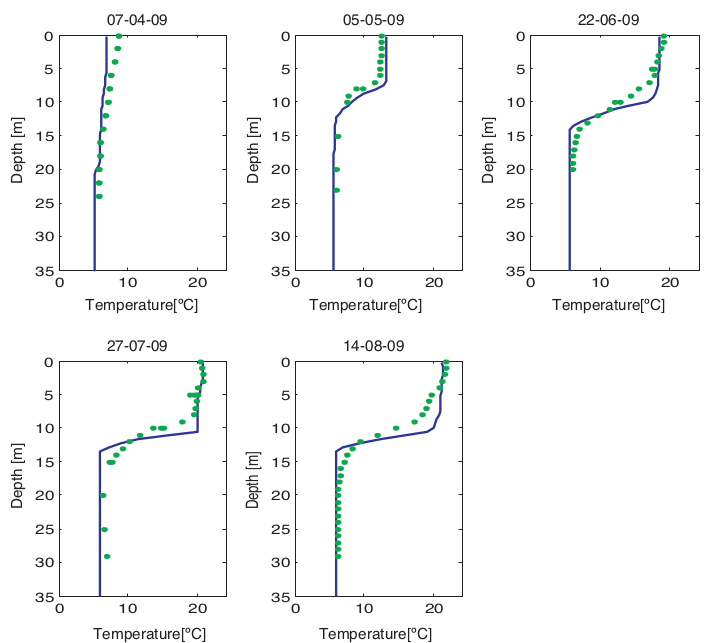
\includegraphics[width=\textwidth]{img/references/medrano2013profiles}
    \caption{Results from \autocite{medrano2013coupling}: the points obtained from the simulations are superimposed to measurements (solid line).}
    \label{fig:medrano2016}
\end{figure}

However, when dealing with phytoplankton blooming, introducing turbulence adds much computational cost to the problem, requiring some other approximations, using the hypotheses of unlimited nutrients and constant rate of loss (\autoref{sec:ref_pla_blooms}). In \autoref{sec:math-model} the mathematical model used in this work is described and commented integrating different formalisms. The most important articles representing the ideal road to this work are reported and commented (\autocite{Sverdrup1953OnPhytoplankton, Huisman2002HowPersist, Taylor2011ShutdownBlooms}). In \autoref{sec:behrenfeld} the \textit{Dilution-Recoupling} hypothesis proposed in \autocite{Behrenfeld2010AbandoningBlooms} is described and discussed with reference to this work.

\subsection{The mathematical model} \label{sec:math-model}
Following \autocite{Shigesada1981AnalysisWaters}, a one-dimensional equation which takes into account all the relevant factors during a bloom follows:
\begin{equation} \label{eq:generic}
    \partial_t n + v \partial_z n = D \partial_z^2 n + (\lambda f - \mu) n
\end{equation}
where \( n = n(z,t) \) is the phytoplankton number density; $t$ is the time coordinate, $z$ is the spacial coordinate (depth); $v$ is the sinking speed of the phytoplankton; $D$ is the effective diffusivity resulting from turbulent motion; \( g = \lambda f - \mu\) is the net growth rate, where $\lambda$ and $\mu$ are constants, related respectively to the production and loss of cells; $f = f(I)$ is a function which modulates the growth rate depending on the light availability $I$. $I = I(n,z)$ is the function which describes light attenuation. Thus, $g = g(I,n,z)$.
\subsubsection{Light income}
The simplest form for light attenuation is linear; a more general form is \(f(I) = a I^\alpha\) \autocite{Ebert2001CriticalBlooms}. A more realistic possibility is to consider \( f(I) = \frac{I}{I+H} \), called a Michaelis-Menten function, which introduces a saturation: for low values of I, the linearity is approached.

The water attenuates the incoming flux in the following way:
\[ \mathrm{d}I = -\bar{k} I \mathrm{d}z \]
Here $\bar{k}$ accounts for two different factors. The first one is the intrinsic attenuation caused by the turbidity of water, which in principle depends on depth, because, being the attenuation coefficient bigger for longer wavelengths, the spectrum of light varies with depth \autocite{Pegau1997AbsorptionSalinity}. However, both because the depth considered is relatively small, and because the most important wavelengths for photosynthesis have a lower attenuation coefficient \footnote{It perhaps makes more sense seen the other way round: the photosynthesis is adapted to the wavelengths which are less attenuated.}, it is a good approximation to consider it constant. The second factor should consider that any cell blocks in some measure the light available to those below it: the resulting attenuation for a given cell is proportional to the number of cells above it. From the equation above \(\bar{k}(z) = k_{bg}z +k_{ss}\int_0^z n(z) \mathrm{d}z\), so
\begin{equation} \label{eq:generic_light}
    I(n,z) = I_0 e^{-k_{bg}z} e^{-k_{ss}\int_0^z n(z) \mathrm{d}z}
\end{equation}
where $I_0$ is the light flux at water surface, $k_{bg}$ accounts for the turbidity of water and $k_{ss}$ models the effect of auto-shading (also called self-shading).


%\begin{equation} \label{eq:full_production}
%    \partial_t n + v \partial_z n = D \partial_z^2 n + \left[ \lambda \frac{I_0 e^{-k_{bg}z - k_{ss} \int_0^z n \mathrm{d}z}}{I_0 e^{-k_{bg}z - k_{ss} \int_0^z n \mathrm{d}z} + H } - %\mu \right] n
%\end{equation}

\subsection{The critical depth hypothesis} \label{sec:sverdrup}
The reference work for the first attempts to model plankton blooming is \autocite{Sverdrup1953OnPhytoplankton}, where under strong assumptions a simple criterion is proposed to predict if water conditions are favourable for such events. The concept of \textit{mixed layer} (ML) is introduced, that is the upper layer, just under the surface of water, where the effective diffusivity is strong enough to make the distribution of phytoplankton cells uniform. The requirement that the net production $g$, integrated over a characteristic time and from the surface to a given depth, be null defines the \textit{critical depth} $h_c$:
\[ G(h) \coloneqq \int_0^T \int_0^{h} g \,\dt\, \dd z\;\;\; ; \;\;\;  G(h_c) = 0\]
In the paper an average value for $I(t)$ is considered, while the present model assumes it is constant, so that the time integral here has no effect. Another, more substantial difference from Sverdrup's model is the form of $f$: no self-shading effect is taken into account and \( f \sim I_0 e^{-k_{bg}z} \). The resulting relation for $h_c$, using these assumptions and the notation of this work, is
\[ \frac{h_c}{1-e^{-k_{bg} h_c}} = -\frac{\lambda I_0}{\mu k_{bg}} \] 
Sverdrup claims that any mixed layer deeper than $h_c$ cannot sustain a bloom, since an uniform mixing would result in a negative growth rate, and discusses this hypothesis with supporting data (but see \autoref{sec:behrenfeld} for a critic discussion). This model is not valid when the diffusivity is weak.

\subsection{The critical turbulence hypothesis} \label{sec:ref_crit_turb}
In order to go beyond the critical depth idea, an explicit dynamical equation analogous to \autoref{eq:generic} is used in \autocite{Huisman2002HowPersist}, where a Michaelis-Menten form is used for $f$ and the self-shading effect is taken into account:
\[ f(I) = \frac{I}{I+H} \;\;;\;\;\;\; I(z,n) = e^{-k_{bg}z-k_{ss}\int_0^zn(z)\mathrm{d}z}\]
In the cited article, numerical methods are developed to determine both the shape of the density of particles in function of depth, and the conditions in which a bloom is possible. The results show a situation where the critical depth condition is met only in the limit of high diffusivity, while in the limit of low diffusivity another depth, the \textit{compensation depth}, represents the maximal depth of the mixed layer before which a bloom can occur; for intermediate values of diffusivity, no maximal depth exists. \\
It is important to discuss how the mixed layer concept relates to the numerical model cited above, since some unrealistic assumptions are made. The model is one-dimensional, limited between $0$ and $h$, and the diffusivity coefficient $D$ is constant in the interval. This means that the mixed layer depth (MLD) is represented by $h$, since all the interval is mixed\footnote{It is indeed a \textit{mixing} layer, which become mixed only when the steady state is reached.}. This is a first approximation: the diffusivity profile is continuous and $D$ has intermediate values before going to zero. The second approximation concerns the boundary conditions: indeed, even considering a step-like mixed layer, a particle is expected to sink linearly once it reaches the bottom of it, while in the model no-flux conditions are imposed (the same condition is imposed at the upper boundary\footnote{Here the condition represents a more realistic assumption: the possibility that a cell be removed from water by wind is of course negligible.}):
\[ J=D\partial_z n - v n \;\; ; \;\;\;\; J_{z=0} = J_{z=h} = 0\]

\subsubsection{Numerical results}
The main results of \autocite{Huisman2002HowPersist} are resumed in \autoref{fig:huisman_Dzplot}: for a sinking phytoplankton species, the critical depth condition described in \autoref{sec:sverdrup} is verified only for high values of diffusivity; intermediate diffusivities can sustain phytoplankton populations no matter how deep the mixing layer is; finally, for diffusivities lower than a minimal value, a \textit{compensation depth} represents the maximal depth of the mixing layer which allows a bloom. When considering a higher sinking velocities, the shape of the plot changes: the ``window'' between the maximal and minimal diffusivities $D_{max}$ and $D_{min}$ closes, making it possible to have blooms only in shallow mixing layers. This effect can be explained looking at the dependence of $D_{min}$ on $v$ (\autoref{eq:D_crit}).
\begin{figure} [ht]
\centering
    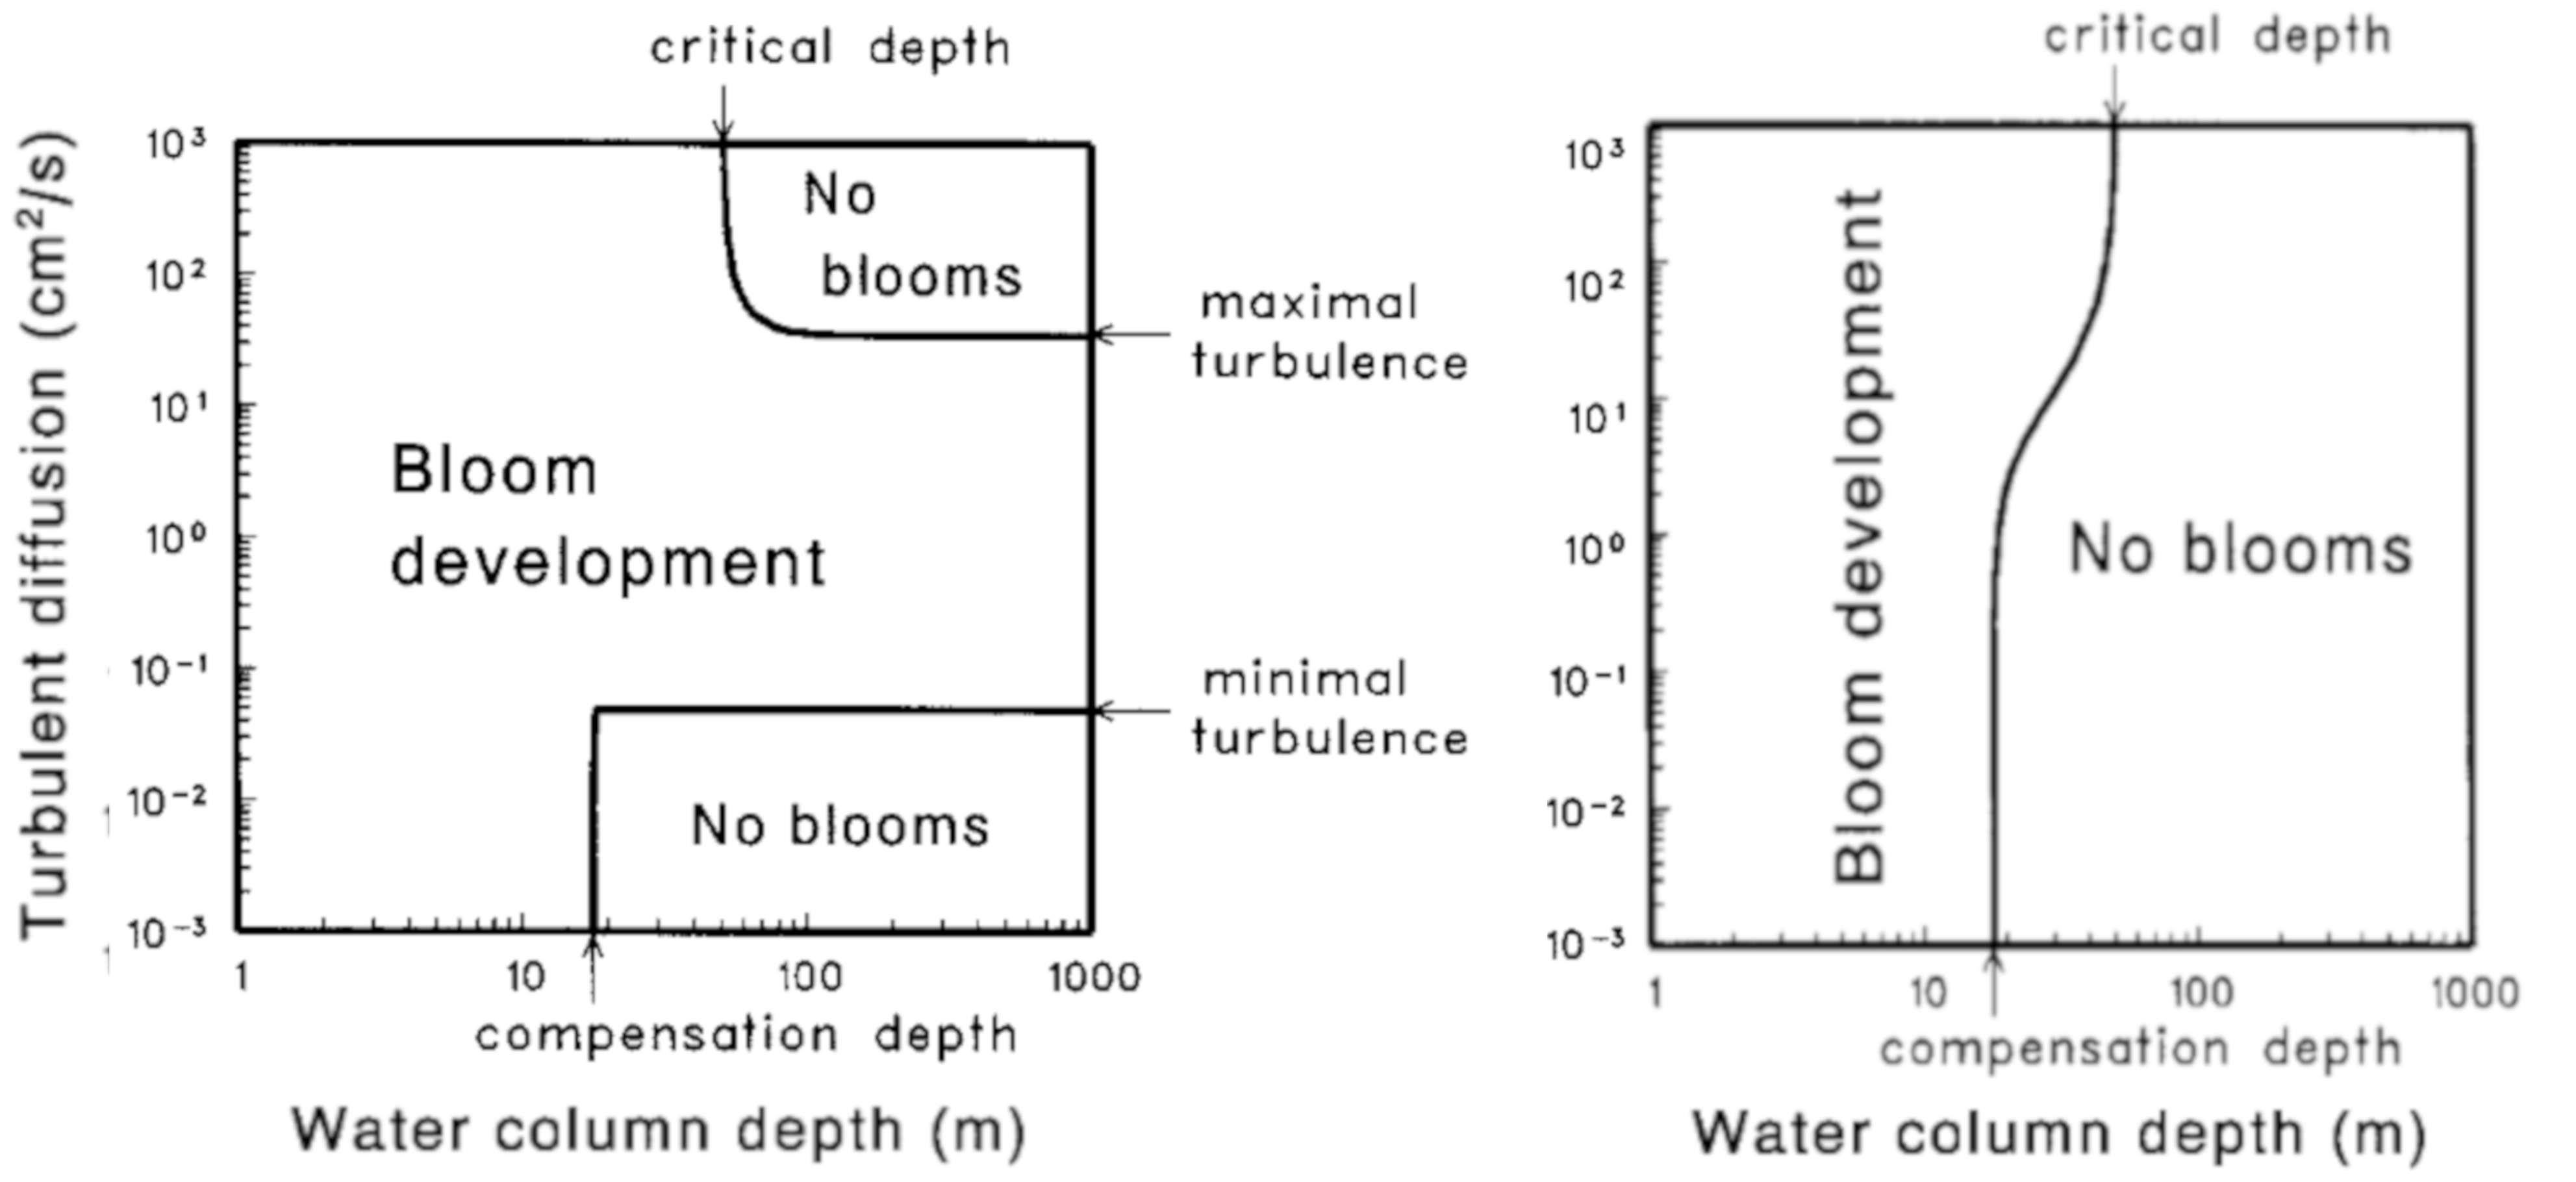
\includegraphics[width=\textwidth]{img/references/huisman2002.png}
    \caption{Blooming conditions: at low sinking velocities, $v=0.04mh^{-1}$ on the left, a bloom can develop only in sufficiently shallow mixed layers, or for intermediate diffusivities; when a higher sinking speed $v$ is considered, $v=0.4mh^{-1}$ on the right, the ``window"" between maximal and minimal diffusivity $D$ closes, due to the dependence on $v$ of the minimal value of $D$. [Image adapted from \autocite{Huisman2002HowPersist}.]}
    \label{fig:huisman_Dzplot}
\end{figure}


\subsubsection{Critical parameters} \label{sec:huism_crit_parameters}
Looking at \autoref{fig:huisman_Dzplot}, the two subsets of points for which there can be no bloom are defined by four quantities: maximal and minimal turbulence $D_{max}$ and $D_{min}$, critical depth $h_c$ and compensation depth $c$. The equation used for the critical depth has already been discussed in \autoref{sec:sverdrup}. An estimate for $c$ can be obtained considering that it is the depth where the growth factor $g$ is null: indeed, in the limit of low $D$, for sinking cells the only way to have a non-decaying density is to have $g(z) \geq 0$ at all depths, since the cells cannot move upwards and would otherwise end up in a decay zone, thus dying. Neglecting the self-shading effect, one have
\[ g(c) = \lambda\frac{1}{\frac{H}{I(c)}} = 0 \Rightarrow
I(c) = \frac{H}{\frac{\lambda}{\mu} -1}\]
Considering that \( I_c = I_0 e^{k_{bg}z} \) it follows
\[ c = \frac{\log{I_0} - \log{I_c}}{k_{bg}} \]
When dealing with $D_{min}$, under the assumptions of non-decaying light intensity and imposing that the cells density be zero at the bottom, following \autocite{riley1949quantitative} it holds:
\[ D_{min} = \frac{v^2}{4g(I_0)} \]
which explains why in \autoref{fig:huisman_Dzplot} the ``window'' closes from below.
Finally, for an estimate of $D_{max}$ one can use the reasoning in \autocite{Taylor2011ShutdownBlooms}: considering a simplified model in which (see \autoref{fig:taylor_simple_model})
\[ g(z) = 
\begin{cases}
    \tilde{\lambda} = \frac{1}{c}\int_0^c (\lambda f(z) - \mu) \mathrm{d}z & \mathrm{if}\; z\leq c \\
    -\mu & \mathrm{if}\; z > c
\end{cases}
\]
The assumption is made that in the upper layer (1) the turbulence is high enough to ensure an uniform solution holds, so that $n_1 = const$. In the lower layer (2), since diffusivity dominates \( D\partial_z^2 n_2 - \mu n_2 = 0 \) (steady-state equation), so that
\begin{equation} \label{eq:n2}
 n_2(z) = \beta e^{\pm\sqrt{\frac{\mu}{D}} z} 
\end{equation}
To match the solutions, 
\begin{equation} \label{eq:n1}
 n_1 = n_2(c) = \beta e^{\pm\sqrt{\frac{\mu}{D}} c}
\end{equation}
At the critical value of $D_{max}$, the downward flux should be exactly compensated by the total production in the upper layer:
\[ \int_0^c \tilde{\lambda} n_1 \mathrm{d}z = D_{max} \partial_z n_2|_{z=c} \]
which substituting the expressions \autoref{eq:n1} and \autoref{eq:n2} becomes
\begin{equation} \label{eq:D_crit}
    D_{max} = \frac{\tilde{\lambda}^2c^2}{\mu}
\end{equation}
Making an approximation and substituting $\tilde{\lambda}$ with its value at the surface, \( \lambda \frac{1}{\frac{H}{I_0}+1} \), this equation can be used to estimate the maximal diffusivity for the model used in this work.


\begin{figure} 
    \centering
  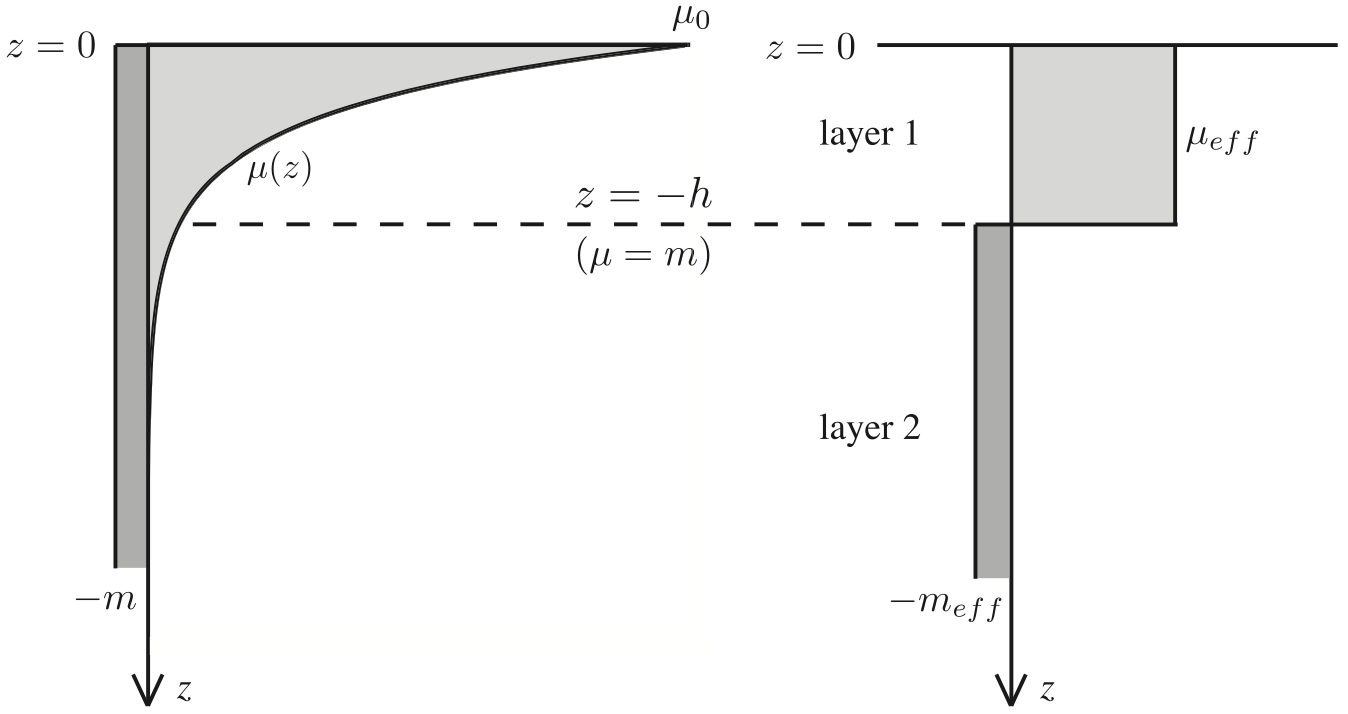
\includegraphics[width=.7\textwidth]{img/references/taylor_simple_model}
  \caption{Visualization of the simple model used in \autocite{Taylor2011ShutdownBlooms} to discuss critical diffusivity. Here a different notation is used: $\mu$ is the reproduction rate, $m$ the loss rate. Instead of an exponentially decaying growth rate, with a constant loss rate (left) one can consider a simple step function.}
  \label{fig:taylor_simple_model}
\end{figure}

\subsection{Mathematical results}
In \autocite{Ebert2001CriticalBlooms}, a mathematical approach allows the analytic determination of the intervals of parameters favourable to blooming, confirming the computational results in \autocite{Huisman1999CriticalBlooms} and \autocite{Huisman1999SpeciesLight}: a simplified form of the production function is used:
\[ f_\alpha(I) = cI^\alpha \]
which can be tuned to approximate the $f$, setting $\alpha$. Actually Ebert refers to the production function \(f_E(I) = \frac{I}{1+cI}\),
which can be however rewritten in terms of $f$:
\[ c\cdot f_E \xleftrightarrow{c=1/H} f \]
A more general choice is to use the adimensional variable \(\phi = \frac{H}{I} = \frac{1}{cI} \) (see \autoref{sec:adimensionalization}):
\[ f(I)|_{I=H/\phi}= H\frac{1}{1+\phi} = Hf(\phi) \]
The asymptotic behaviour is as follows:
\begin{equation}
    f(\phi) = \frac{1}{1+\phi} \simeq
    \begin{cases}
        \phi^{-1} - \phi^{-2} & \mathrm{if}\; \phi \gg 1 \\
        1 - \phi & \mathrm{if}\; \phi \ll 1
    \end{cases}
\end{equation}

In the limit of high $\phi$, it is useful to use the auxiliary variable \( \psi = \phi^{-1}\), so that \( f(\phi) = f(1/\psi) \sim_0 \psi - \psi^2\). The function is then well approximated by $f_\alpha(\psi) = \psi ^\alpha $, with \(\alpha\in\;]0,1]\). In particular, if \(\psi \rightarrow 0 \) the best choice is \( \alpha \sim 1 \). Another approach is minimizing the integral of the difference \( \Delta(\psi,\alpha) := f_\alpha(\psi) - f(\psi) \) between $0$ and a small value $\bar{\psi}$\footnote{Since $\Delta>0$ for \(0<\alpha<1\), there is no need to take the absolute value.}: 
\[ \mathcal{I}(\alpha) = \int_0^{\bar{\psi}} \Delta(\psi,\alpha) =\frac{\bar{\psi}^{\alpha+1}}{\alpha} -\frac {\bar{\psi}^2}{2} + \frac{\bar{\psi}^3}{3} \]
Imposing that the derivative is null in $\tilde{\alpha}$, it results \(\tilde{\alpha} = \frac{1}{\log\bar{\psi}} \).

\begin{figure} [ht]
    \centering
    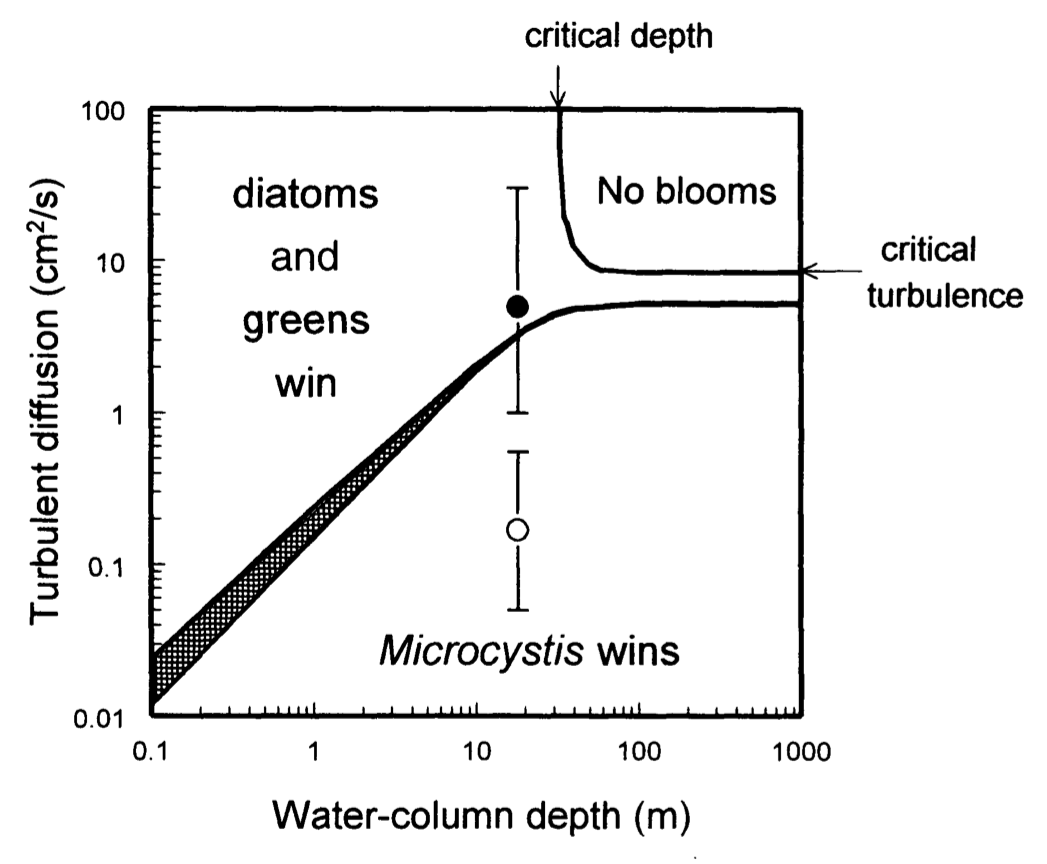
\includegraphics[width=.7\textwidth]{img/references/huisman2004}
    \caption{Using the prediction of \autocite{Ebert2001CriticalBlooms} and \autocite{Huisman2002HowPersist}, this plot from \autocite{Huisman2004ChangesSpecies} shows three possible outcomes depending on the diffusivity and depth of water: when the mixing is sufficiently high, the sinking species are advantaged, otherwise the buoyant cyanobacteria prevail; over the critical depth and the critical turbulence, no bloom can develop. The two points, with error bars upon diffusivity due to its difficult measure, represent the lake conditions before (white point) and after (black point) increasing mixing.} 
    \label{fig:huisman2004}
\end{figure}
In \autocite{Huisman2004ChangesSpecies}, this model goes one step further, studying the competition between two species, one buoyant (the cyanobacterium \textit{Microcystis}), and one sinking (grouping diatoms, mainly of genera \textit{Cyclotella} and \textit{Stefanodiscus}, and green algae, mainly in genus \textit{Scenedesmus}). The predictions coming from the one-dimensional model are applied to experimental data, as shown in \autoref{fig:huisman2004}: in agreement with data, varying the mixing of the lake results in a shift in the composition of the bloom, from harmful cyanobacteria to diatoms and green algae.
Other experimental results are reported in  \autocite{Visser2016ArtificialReview}: the artificial mixing has proven to be effective in regulating blooms.

\subsection{Heat flow critical forcing}
A complementary approach to the critical turbulence criterion is proposed in \autocite{Taylor2011ShutdownBlooms}, where the turbulence is correlated to the forcing given by the heat flux: in spring, the air temperature increases and the flux from water reduces; this is correlated with a decreased stratification of temperature, suppressing the mixing. The paper reports both a theoretical dissertation and the results of simulation. The Large Eddy Simulation (LES) approach is used, where the Navier-Stokes equation are explicitly resolved only down to a chosen energy, thus neglecting the less energetic modes, but allowing a larger-scale insight. A graphical comparison between the measured chlorophyll concentration (marker of phytoplankton) and surface heat flux concludes the paper: the agreement between the hypothesis and the data is visually evident.
This approach is particularly interesting because, although the underlying mechanism is the same as in the critical turbulence hypothesis, proposes a different observable to predict the blooms, namely the heat flux, which is indeed easier to measure than the effective diffusivity\footnote{For instance, at \url{https://iridl.ldeo.columbia.edu/SOURCES/.SOC/.GASC97/.hfns/\#info} 
a global dataset of heat flux can be found.}. 

\subsection{The Dilution-Recoupling hypothesis} \label{sec:behrenfeld}
In \autocite{Behrenfeld2010AbandoningBlooms} a different approach from the previous has been proposed, definitely criticizing the Critical Depth hypothesis and actually attributing the onset of bloom to mechanisms other than the light income limitation. The paper backs this claims up with satellite data and in particular it negates Sverdrup's hypothesis noting that there are cases in which $C_{phyt}$ shows an increase \textit{before} the MLD shows a shoaling, or even decreases without the ML deepening. Even if \autoref{fig:behrenfeld2010alldata} shows an agreement of phytoplankton biomass variation with both PAR and MLD variations, apparently confirming Sverdrup's hypothesis. In \autocite{Behrenfeld2010AbandoningBlooms}, however, a deeper analysis leads to evaluate the growth factor $g$, showing that its increase begins without correspondence to PAR increasing or ML shoaling (\autoref{fig:behrenfeld2010r}).

\begin{figure} [H]
    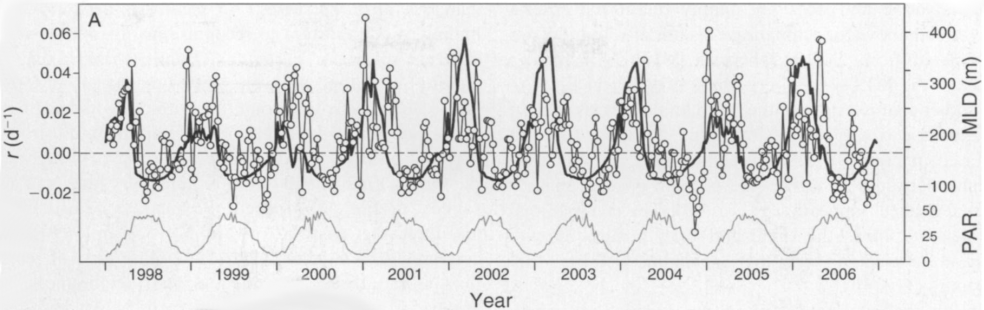
\includegraphics[width=\textwidth]{img/references/behrenfeld2010r}
    \caption{This data visualization, taken from \autocite{Behrenfeld2010AbandoningBlooms}, shows the growth factor (here $r$, white dots), MLD (heavy black line) and PAR (light line) over a period of nine years.}
    \label{fig:behrenfeld2010r}
\end{figure}

The model used take into account different loss factors: grazing by zooplankton ($\mu_{graz}$), sinking loss, death caused by viruses or parasites, flush loss due to dilution processes\footnote{Flush and sinking losses are related to the absorbing conditions in \autoref{sec:stoc_boundaries}.}.

The hypothesis describes two phases: in the first one, a deepening of the ML dilutes the plankton populations, reducing the encounter rate of grazers with phytoplankton, thus decreasing the influence that an increase in biomass would have with respect to the grazing losses (\textit{decoupling} of $\lambda$ and $\mu_{graz}$); in the second one, the MLD stabilizes and with the increase of phytoplankton density the encounter rate increases again (\textit{recoupling}). This processes respectively increase and decrease the growth factor $g$, thus ruling out the Critical Depth hypothesis; moreover, a shoaling of the ML would actually further accelerate the recoupling, with very different consequences from the ones claimed by Sverdrup.

Would this hypothesis be proven right, it would nevertheless not mean that the model in \autocite{Shigesada1981AnalysisWaters} and the results in \autocite{Huisman2002HowPersist} are wrong, but simply that their conditions are not determining the onset of blooms. In other words, their constraints would be valid, the critical parameters existing within them. Furthermore, the Critical Turbulence hypothesis has proven to be valid at least in lakes and water basins (\autocite{Visser2016ArtificialReview}, \autocite{Huisman2004ChangesSpecies}), allowing to predict and control the blooming of phytoplankton and therefore remaining a valid and useful tool.